\documentclass[12pt,letterpaper]{article}

% ============================================================================
% PAQUETES ESTÁNDAR DE LATEX (CODIFICACIÓN UTF-8 Y ESPAÑOL)
% ============================================================================
\usepackage[utf8]{inputenc}
\usepackage[T1]{fontenc}
\usepackage[spanish,es-tabla,es-noshorthands]{babel}
\usepackage{amsmath}
\usepackage{geometry}
\usepackage{graphicx}
\usepackage{xcolor}
\usepackage{booktabs}
\usepackage{longtable}
\usepackage{array}
\usepackage{enumitem}
\usepackage{fancyhdr}
\usepackage{titlesec}
\usepackage{tcolorbox}
\usepackage{float}
\usepackage{hyperref}

\geometry{
  letterpaper,
  top=2.5cm,
  bottom=2.5cm,
  left=2.5cm,
  right=2.5cm,
  headheight=15pt
}

% ============================================================================
% PALETA DE COLORES CORPORATIVOS DE CHOCOARTISAN
% ============================================================================
\definecolor{cacaoprofundo}{HTML}{3E2723}
\definecolor{cacaooscuro}{HTML}{261512}
\definecolor{cremacacao}{HTML}{FFF8E1}
\definecolor{doradoimperial}{HTML}{D4AF37}
\definecolor{verdexito}{HTML}{2E7D32}

\hypersetup{
  colorlinks=true,
  linkcolor=cacaoprofundo,
  urlcolor=cacaoprofundo,
  citecolor=cacaoprofundo,
  pdftitle={02\_App - ChocoArtisan Fase I - Programacion Web UIS},
  pdfauthor={Alejandro Sanabria, Jhon Cardenas, Jesus Parada, Deissy Romero}
}

% Configuración de encabezados y pies de página
\pagestyle{fancy}
\fancyhf{}
\fancyhead[L]{\textcolor{cacaoprofundo}{\textbf{ChocoArtisan — Plataforma Web Corporativa y Tienda en Línea (Fase I)}}}
\fancyhead[R]{\textcolor{cacaoprofundo}{\textbf{Grupo 02 — UIS}}}
\fancyfoot[L]{\textcolor{gray}{\small Programación Web — Ing. Manuel Florez}}
\fancyfoot[R]{\textcolor{cacaoprofundo}{\textbf{Página \thepage}}}
\renewcommand{\headrulewidth}{0.6pt}
\renewcommand{\footrulewidth}{0.4pt}

% Formato de títulos de sección
\titleformat{\section}
  {\Large\bfseries\color{cacaoprofundo}}
  {\thesection.}{0.6em}{}[\titlerule]

\titleformat{\subsection}
  {\large\bfseries\color{cacaoprofundo}}
  {\thesubsection}{0.6em}{}

\begin{document}

% ============================================================================
% 1. PORTADA INSTITUCIONAL
% ============================================================================
\begin{titlepage}
  \centering
  \vspace*{0.4cm}
  {\Large\bfseries\textcolor{cacaoprofundo}{UNIVERSIDAD INDUSTRIAL DE SANTANDER (UIS)}\par}
  \vspace{0.2cm}
  {\large\bfseries FACULTAD DE INGENIERÍA — ESCUELA DE INGENIERÍA DE SISTEMAS E INFORMÁTICA\par}
  \vspace{0.2cm}
  {\normalsize ASIGNATURA: PROGRAMACIÓN WEB — FASE I (DESARROLLO FRONTEND EN REACT)\par}

  \vspace{1.0cm}
  
\includegraphics[width=4.4cm]{../ProyectoProgramacionWeb/src/multimedia/imagenes/logo_chocoartisan.png}
  \vspace{0.8cm}

  \begin{tcolorbox}[
    colback=cremacacao,
    colframe=cacaoprofundo,
    boxrule=1.8pt,
    arc=6pt,
    width=0.95\textwidth
  ]
    \centering
    \vspace{0.3cm}
    {\LARGE\bfseries\textcolor{cacaoprofundo}{PROYECTO DE PROGRAMACIÓN WEB — GRUPO 02}\par}
    \vspace{0.35cm}
    {\Huge\bfseries\textcolor{cacaooscuro}{ChocoArtisan:}\par}
    \vspace{0.2cm}
    {\Large\bfseries\textcolor{cacaoprofundo}{Plataforma Web Corporativa y Tienda en Línea para Chocolatería Artesanal}\par}
    \vspace{0.25cm}
    {\normalsize\textit{Reporte Técnico de Implementación Fase I en React.js, React Router y React-Bootstrap}\par}
    \vspace{0.3cm}
  \end{tcolorbox}

  \vspace{1.0cm}
  {\large\bfseries Integrantes del Equipo de Desarrollo:\par}
  \vspace{0.3cm}
  \begin{tabular}{ll}
    \textbf{1. Alejandro Sanabria Zúñiga} & \textit{(Líder de Grupo — Arquitectura y Rutas)} \\
    \textbf{2. Jhon Bayron Cárdenas Camacho} & \textit{(Diseño UI/UX, Maquetación y Responsividad)} \\
    \textbf{3. Jesús David Parada Palencia} & \textit{(Desarrollo React y Carrito Interactivo)} \\
    \textbf{4. Deissy Liliana Romero Prada} & \textit{(Seguridad Captcha y Configurador 3D/2D)} \\
  \end{tabular}

  \vfill
  {\large\textbf{Docente:}\par}
  {\large Ing. Manuel Florez\par}
  \vspace{0.5cm}
  {\normalsize Bucaramanga, Santander — Octubre de 2026\par}
\end{titlepage}

% Tabla de contenido
\tableofcontents
\newpage

% ============================================================================
% 2. OBJETIVOS GENERALES Y ESPECÍFICOS DE LA APLICACIÓN
% ============================================================================
\section{Objetivos de la Aplicación Web ChocoArtisan}

\begin{tcolorbox}[colback=cremacacao,colframe=doradoimperial,title=\textbf{Nota Aclaratoria sobre el Alcance de los Objetivos},coltitle=cacaooscuro,fonttitle=\bfseries]
Los objetivos formulados a continuación corresponden exclusivamente al propósito funcional, comercial y tecnológico del aplicativo web \textbf{ChocoArtisan} como plataforma de comercio electrónico de chocolatería artesanal gourmet, diferenciándose de los objetivos pedagógicos de la asignatura.
\end{tcolorbox}

\subsection{Objetivo General de la Aplicación}
\begin{itemize}[leftmargin=1.2cm]
  \item Desarrollar \textbf{ChocoArtisan}, un sitio web corporativo y tienda de comercio electrónico (\textit{e-commerce}) interactivo para una marca premium de chocolatería artesanal santandereana, integrando una interfaz de usuario elegante, minimalista y responsiva en el \textit{Frontend} mediante \textbf{React.js}, \textbf{React-Bootstrap} y \textbf{React Router}, con gestión dinámica de catálogo, carrito de compras automatizado, personalización de cajas de bombones en 3D/2D y control de acceso mediante rutas públicas y privadas protegidas.
\end{itemize}

\subsection{Objetivos Específicos de la Aplicación}
\begin{enumerate}[leftmargin=1.2cm]
  \item \textbf{Diseñar una interfaz gráfica web responsiva, elegante y accesible} empleando una paleta de colores corporativos inspirada en el cacao (\textit{café profundo} \texttt{\#3E2723}, \textit{crema} \texttt{\#FFF8E1}, \textit{dorado imperial} \texttt{\#D4AF37} y \textit{blanco puro} \texttt{\#FFFFFF}), estructurada con maquetación a tres columnas en la portada, barra de navegación fija (\texttt{fixed-top}), tipografía capitular (\texttt{::first-letter}) y adaptabilidad completa para teléfonos celulares, tablets y computadores de escritorio (\textit{Desktop}).
  \item \textbf{Implementar un sistema de enrutamiento seguro en cliente (\texttt{react-router-dom})} que separe estrictamente las \textbf{rutas públicas} de las \textbf{rutas privadas}, impidiendo el ingreso no autorizado por puertas traseras (\textit{backdoors}) y desplegando el \textit{Menú de Rutas Privadas} únicamente tras verificar las credenciales en una ventana \texttt{Modal} de Bootstrap (patrón de prueba \texttt{login: Admin} | \texttt{passwd: 1234}).
  \item \textbf{Desarrollar componentes interactivos de comercio electrónico en React} para el filtrado en tiempo real del catálogo de productos por categorías (\textit{Bombones de Autor, Barras Finitas de Origen, Cajas de Regalo, Trufas y Ediciones Especiales}) y la liquidación automática del carrito de compras (cálculo de Subtotal, Impuestos IVA del 19\%, tarifas de envío dinámico según la ciudad de destino y cupones de descuento promocionales).
  \item \textbf{Incorporar un módulo de registro de clientes seguro} construido con \texttt{react-bootstrap/Form} que valide en tiempo real la fortaleza criptográfica de las contraseñas (mínimo 8 caracteres, al menos una letra mayúscula, un número y un carácter especial) e integre un mecanismo \textbf{Captcha interactivo anti-bots}.
  \item \textbf{Construir el configurador interactivo ``Crea tu Caja de Chocolates Personalizada'' (3D/2D)} como aporte innovador del equipo de trabajo, permitiendo al usuario elegir cofres de 6, 12 o 24 cavidades, seleccionar individualmente cada bombón o trufa, visualizar la caja en perspectiva 3D o vista 2D y recalcular el precio en tiempo real.
\end{enumerate}

\newpage

% ============================================================================
% 3. IMAGEN: COPIA DE LA PRIMERA PÁGINA DEL SITIO FASE-I
% ============================================================================
\section{Imagen: Copia de la Primera Página del Sitio (Fase-I)}

A continuación se presenta la captura real de la página principal (Portada Fase-I) del aplicativo \textbf{ChocoArtisan} ejecutándose en el navegador web. En ella se aprecia la barra de navegación fija superior con el logo y botón de Login, el \textit{Hero Banner} corporativo, el Carrusel promocional, el diseño a tres columnas con recursos multimedia (Video, Sonido, Acordeón, letra capitular y efectos Bootstrap), la vitrina del catálogo y el formulario de despacho:

\begin{figure}[H]
  \centering
  \fbox{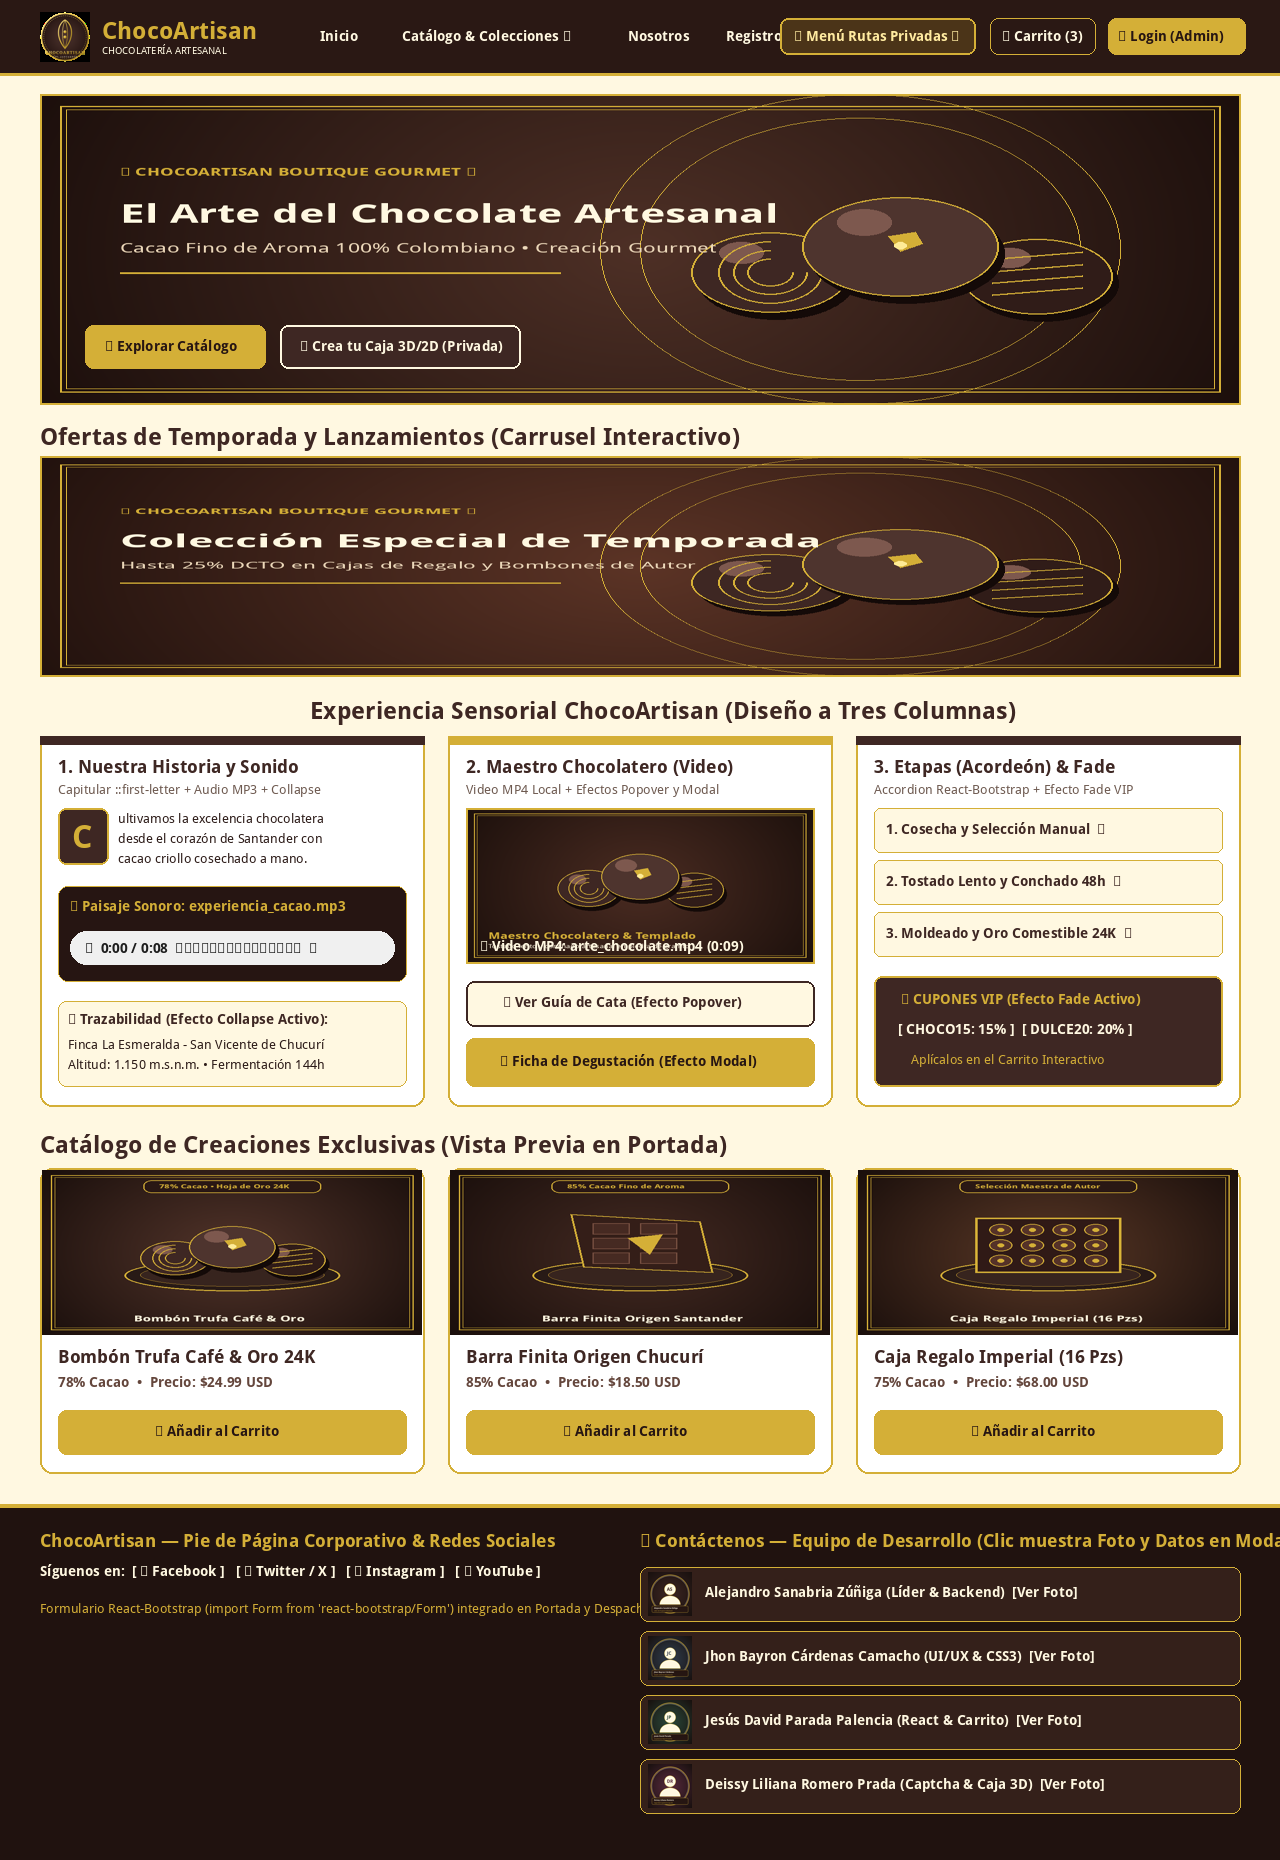
\includegraphics[width=0.92\textwidth,height=13.2cm,keepaspectratio]{captura_portada_fase1.png}}
  \caption{Copia de la primera página (Portada Fase-I) del sitio web ChocoArtisan en ejecución.}
  \label{fig:portada_fase1}
\end{figure}

\begin{figure}[H]
  \centering
  \begin{minipage}{0.48\textwidth}
    \centering
    \fbox{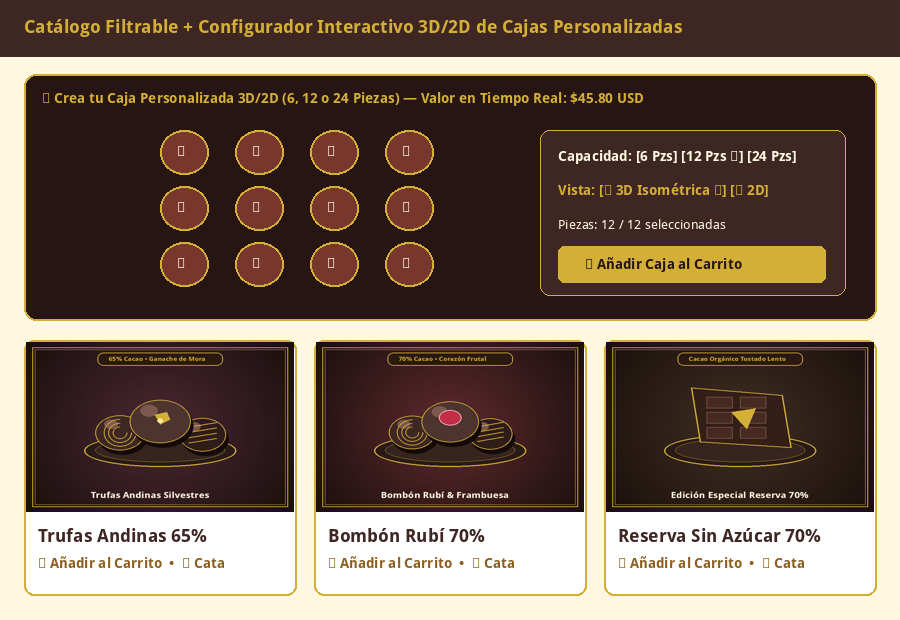
\includegraphics[width=0.96\textwidth]{captura_catalogo.png}}
    \caption{Vista del Catálogo Interactivo filtrable por categorías y pureza de cacao.}
  \end{minipage}\hfill
  \begin{minipage}{0.48\textwidth}
    \centering
    \fbox{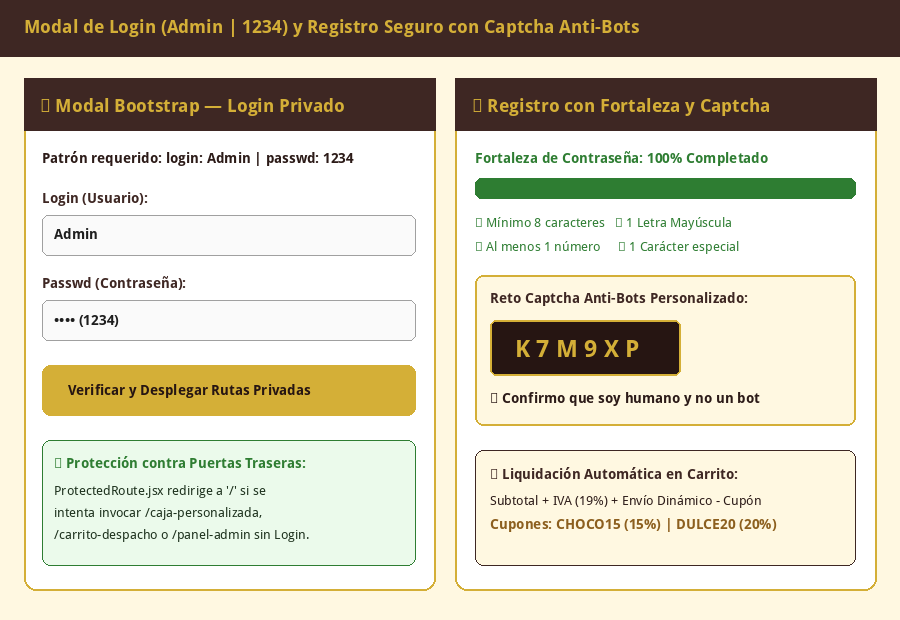
\includegraphics[width=0.96\textwidth]{captura_registro_captcha.png}}
    \caption{Módulo de Registro de Clientes con validación de contraseña y Captcha.}
  \end{minipage}
\end{figure}

\newpage

% ============================================================================
% 4. ESTRUCTURA JERÁRQUICA DEL SITIO EN EL DISCO
% ============================================================================
\section{Estructura Jerárquica del Sitio en el Disco}

El proyecto se ha organizado siguiendo una arquitectura modular limpia en la que las hojas de estilo (\texttt{styles/}), los componentes React documentados (\texttt{components/}), los archivos de datos (\texttt{data/}) y los recursos multimedia (\texttt{multimedia/imagenes}, \texttt{multimedia/sonido}, \texttt{multimedia/videos}) residen en carpetas separadas y claramente estructuradas.

\subsection{Imagen de la Estructura Jerárquica en el Disco}

\begin{figure}[H]
  \centering
  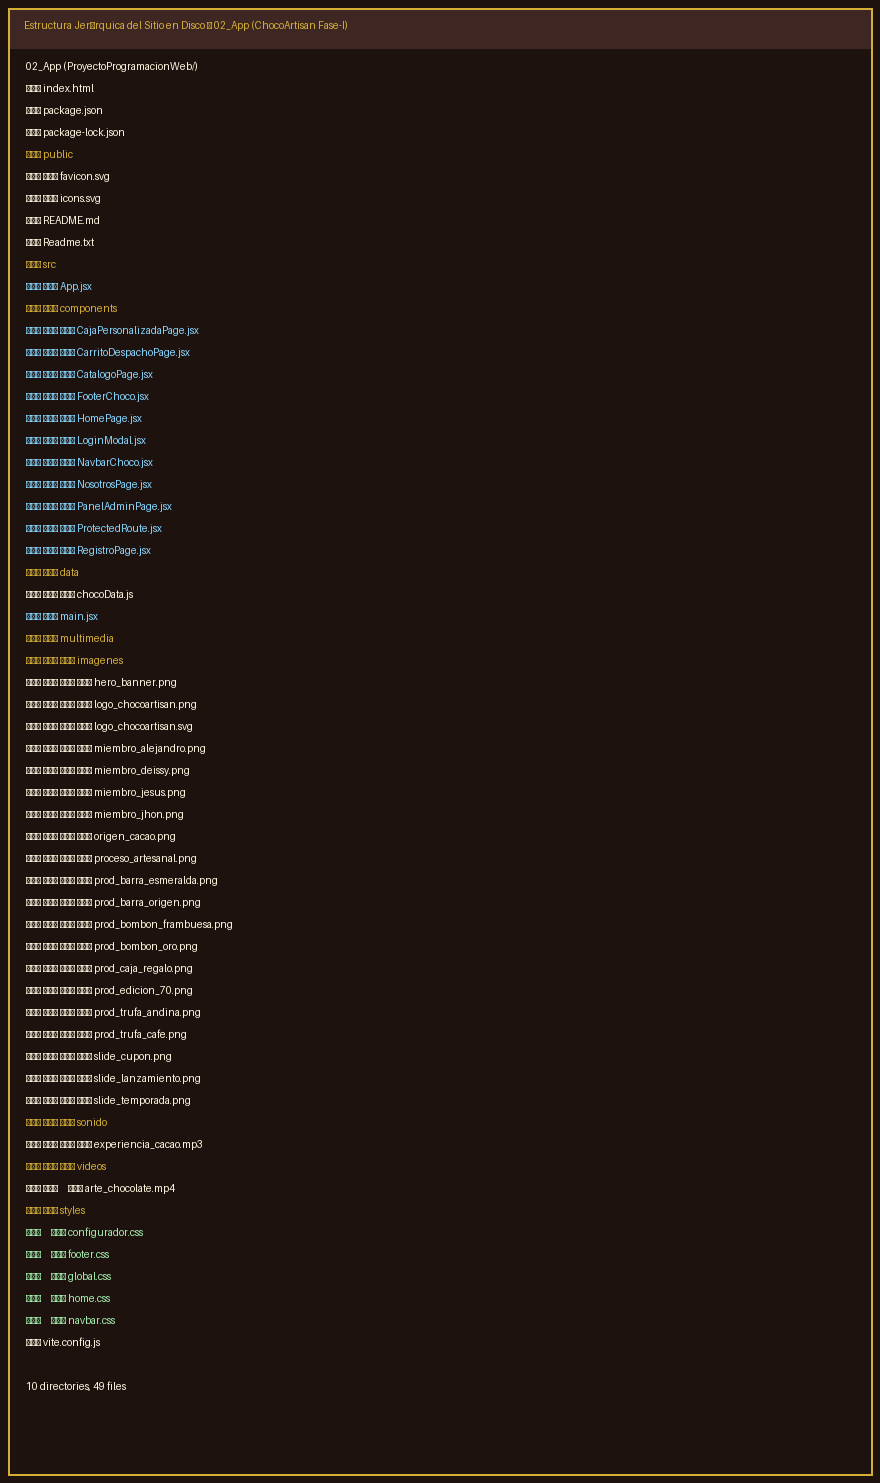
\includegraphics[width=0.88\textwidth]{estructura_jerarquica_disco.png}
  \caption{Fotografía/captura del árbol jerárquico de carpetas y archivos en disco (\texttt{02\_App / ProyectoProgramacionWeb}) sin incluir \texttt{node\_modules}.}
  \label{fig:estructura_disco}
\end{figure}

\subsection{Explicación del Significado de Cada Carpeta, Subcarpeta y Archivo}

\begin{longtable}{p{0.34\textwidth} p{0.61\textwidth}}
\toprule
\textbf{Carpeta / Archivo} & \textbf{Significado y Responsabilidad Técnica en el Aplicativo} \\
\midrule
\endhead
\texttt{ProyectoProgramacionWeb/} & Directorio raíz del aplicativo React correspondiente a la entrega \texttt{02\_App} de la Fase I. \\
\midrule
\texttt{index.html} & Plantilla HTML5 base donde se monta el nodo raíz \texttt{<div id="root">} del DOM virtual de React y se define el título e idioma (\texttt{lang="es"}). \\
\midrule
\texttt{package.json} & Manifiesto del proyecto Node/NPM que declara las dependencias de producción (\texttt{react}, \texttt{react-dom}, \texttt{react-router-dom}, \texttt{react-bootstrap}, \texttt{bootstrap}) y los scripts (\texttt{dev}, \texttt{build}, \texttt{lint}). \\
\midrule
\texttt{vite.config.js} & Archivo de configuración del empaquetador y servidor de desarrollo ultrarrápido Vite con soporte para React y Babel. \\
\midrule
\texttt{Readme.txt} & Manual paso a paso detallado para instalar dependencias (\texttt{npm install}), ejecutar en local (\texttt{npm run dev}) y desplegar en servidor de producción. \\
\midrule
\texttt{public/} & Carpeta de activos estáticos servidos en la raíz del dominio (\texttt{favicon.svg}, \texttt{icons.svg}). \\
\midrule
\texttt{src/} & Carpeta principal del código fuente de la aplicación React. \\
\midrule
\texttt{src/main.jsx} & Punto de entrada de React (\texttt{createRoot}) que inyecta las hojas de estilo de Bootstrap 5 (\texttt{bootstrap.min.css}), \texttt{global.css} y el componente \texttt{App.jsx}. \\
\midrule
\texttt{src/App.jsx} & Componente raíz que configura \texttt{BrowserRouter}, administra el estado global (sesión de Login, carrito de compras, órdenes y usuarios) y declara las Rutas Públicas y Privadas. \\
\midrule
\texttt{src/components/} & \textbf{Subcarpeta de Scripts JSX (Componentes):} Aloja todos los módulos de interfaz y páginas documentados con comentarios JSDoc. \\
\quad \texttt{NavbarChoco.jsx} & Barra de navegación superior fija (\texttt{fixed="top"}) con logo, enlaces públicos, submenú \texttt{Dropdown} de colecciones y el \textit{Menú de Rutas Privadas} que se despliega al iniciar sesión. \\
\quad \texttt{LoginModal.jsx} & Ventana \texttt{Modal} de Bootstrap con \texttt{import Form from 'react-bootstrap/Form'} que valida el patrón \texttt{login: Admin} | \texttt{passwd: 1234}. \\
\quad \texttt{ProtectedRoute.jsx} & Guardia de seguridad para rutas privadas que bloquea accesos directos por URL (\textit{puertas traseras}), redirigiendo a \texttt{"/"} si el usuario no se ha autenticado. \\
\quad \texttt{HomePage.jsx} & Portada principal con Hero Banner, Carrusel, diseño a tres columnas, Video, Sonido, Acordeón, letra capitular y efectos \texttt{Collapse}, \texttt{Popover}, \texttt{Modal} y \texttt{Fade}. \\
\quad \texttt{CatalogoPage.jsx} & Catálogo interactivo filtrable por las 5 categorías oficiales, barra de búsqueda y deslizador de porcentaje de cacao. \\
\quad \texttt{NosotrosPage.jsx} & Página corporativa con la historia de ChocoArtisan, trazabilidad del cacao santandereano, pilares de sostenibilidad y preguntas frecuentes. \\
\quad \texttt{RegistroPage.jsx} & Formulario de registro de clientes con barra de progreso de fortaleza de contraseña y componente \textbf{Captcha interactivo anti-bots}. \\
\quad \texttt{CajaPersonalizadaPage.jsx} & \textit{(Ruta Privada)} Configurador interactivo 3D/2D ``Crea tu Caja de Chocolates Personalizada'' de 6, 12 o 24 piezas con cálculo de precio en tiempo real. \\
\quad \texttt{CarritoDespachoPage.jsx} & \textit{(Ruta Privada)} Carrito de compras interactivo con cálculo de Subtotal, cupones de descuento, IVA (19\%), envío dinámico por ciudad y formulario de despacho. \\
\quad \texttt{PanelAdminPage.jsx} & \textit{(Ruta Privada)} Panel administrativo que consolida el inventario de productos, las órdenes generadas y los clientes verificados. \\
\quad \texttt{FooterChoco.jsx} & Pie de página con los 4 integrantes del equipo (al hacer clic despliega un \texttt{Modal} con foto y datos básicos del estudiante) y enlaces a 4 redes sociales. \\
\midrule
\texttt{src/styles/} & \textbf{Subcarpeta de Hojas de Estilo CSS:} Contiene la maquetación separada por responsabilidades y comentada. \\
\quad \texttt{global.css} & Variables CSS de la paleta cacao, reglas de letra capitular (\texttt{.drop-cap-choco::first-letter}) y \textit{media queries} para celulares, tablets y Desktop. \\
\quad \texttt{navbar.css} & Estilos para la barra fija superior, menús desplegables y resaltado dorado del menú privado. \\
\quad \texttt{home.css} & Estilos del Hero Banner, Carrusel, cajas del diseño a tres columnas y tarjetas del catálogo. \\
\quad \texttt{configurador.css} & Transformaciones CSS3 con perspectiva isométrica 3D (\texttt{rotateX}, \texttt{rotateZ}) y grillas de 6, 12 y 24 cavidades. \\
\quad \texttt{footer.css} & Estilos del pie de página, tarjetas interactivas de estudiantes y botones de redes sociales. \\
\midrule
\texttt{src/data/chocoData.js} & Módulo de datos estructurados con los 8 productos del catálogo, piezas del configurador 3D, cupones, tarifas de envío y fichas de los 4 integrantes del equipo. \\
\midrule
\texttt{src/multimedia/} & \textbf{Subcarpeta de Recursos Multimedia:} Organizada en tres subdirectorios especializados: \\
\quad \texttt{imagenes/} & Contiene 19 imágenes locales en formato PNG/SVG: logo corporativo, banners del carrusel, fotografías ilustradas de los 8 productos, origen/proceso y fotos de perfil de los 4 estudiantes. \\
\quad \texttt{sonido/} & Contiene el archivo de audio \texttt{experiencia\_cacao.mp3} reproducido en la primera columna de la portada. \\
\quad \texttt{videos/} & Contiene el video \texttt{arte\_chocolate.mp4} (codificado en H.264/AAC) sobre el proceso artesanal del chocolate. \\
\bottomrule
\end{longtable}

\newpage

% ============================================================================
% 5. EXPLICACIÓN DE TODAS LAS FUNCIONALIDADES IMPLEMENTADAS (MENÚS Y SUB-MENÚS)
% ============================================================================
\section{Explicación de Todas las Funcionalidades Implementadas (Menús y Sub-menús)}

\subsection{Barra de Navegación Fija (\texttt{NavbarChoco.jsx}) y Arquitectura de Menús}
La barra de navegación superior utiliza la propiedad \texttt{fixed="top"} de \texttt{react-bootstrap}, garantizando que permanezca siempre visible e inamovible en la parte superior de la pantalla sin importar a qué página se navegue o cuánto desplazamiento vertical (\textit{scroll}) realice el usuario. Su estructura se divide en:

\begin{enumerate}[leftmargin=1.2cm]
  \item \textbf{Menú Principal de Rutas Públicas (Accesible a todo visitante):}
    \begin{itemize}
      \item \textbf{Inicio (\texttt{/}):} Dirige a la portada integral de Fase I.
      \item \textbf{Sub-menú Desplegable ``Catálogo \& Colecciones'' (Efecto \texttt{Dropdown}):} Implementado con \texttt{NavDropdown} de \texttt{react-bootstrap}. Despliega seis opciones de filtrado directo:
        \begin{itemize}
          \item \textit{Ver Todo el Catálogo}
          \item \textit{Bombones de Autor}
          \item \textit{Barras Finitas de Origen}
          \item \textit{Cajas de Regalo}
          \item \textit{Trufas}
          \item \textit{Ediciones Especiales}
        \end{itemize}
      \item \textbf{Nosotros (\texttt{/nosotros}):} Invoca la sección corporativa con la historia de la chocolatería, el origen del cacao santandereano y los procesos de elaboración.
      \item \textbf{Registro (Captcha) (\texttt{/registro}):} Invoca el formulario de creación de cuentas con validador de contraseñas y filtro anti-bots.
    \end{itemize}

  \item \textbf{Autenticación en Modal (\texttt{LoginModal.jsx}) y Despliegue del Menú de Rutas Privadas:}
    \begin{itemize}
      \item Al pulsar el botón dorado \textbf{``Login (Admin | 1234)''}, se abre un componente \texttt{Modal} de Bootstrap que implementa el patrón exigido \texttt{login: xxxxxx; passwd: xxxxxxx} empleando \texttt{import Form from 'react-bootstrap/Form';}.
      \item Al verificar exitosamente las credenciales de prueba (\textbf{Usuario:} \texttt{Admin} | \textbf{Contraseña:} \texttt{1234}) o cualquier cuenta creada en el módulo de registro, el estado global \texttt{isAuthenticated} pasa a \texttt{true} y se despliega dinámicamente en la barra superior el sub-menú dorado \textbf{``Menú Rutas Privadas''}.
      \item \textbf{Sub-menús de Rutas Privadas:}
        \begin{enumerate}
          \item \textbf{Configurador Caja 3D/2D (\texttt{/caja-personalizada}):} Acceso al configurador interactivo de cajas de 6, 12 y 24 piezas.
          \item \textbf{Carrito Interactivo y Despacho (\texttt{/carrito-despacho}):} Acceso a la liquidación financiera del pedido y guía de envío.
          \item \textbf{Panel de Órdenes e Inventario (\texttt{/panel-admin}):} Vista administrativa de órdenes registradas, stock de productos y clientes verificados.
        \end{enumerate}
    \end{itemize}

  \item \textbf{Protección contra Entradas por Puertas Traseras (\texttt{ProtectedRoute.jsx}):}
    \begin{itemize}
      \item Si un usuario no autenticado intenta escribir manualmente en la barra de direcciones del navegador una ruta privada (por ejemplo, \texttt{http://localhost:5173/caja-personalizada} o \texttt{/panel-admin}), el componente guardia \texttt{ProtectedRoute} intercepta la petición, impide el renderizado del componente privado, redirige automáticamente a la raíz \texttt{"/"} mediante \texttt{<Navigate to="/" replace />} y abre el Modal de Login con una alerta de seguridad.
    \end{itemize}
\end{enumerate}

\subsection{Diseño a Tres Columnas, Multimedia y Efectos de Bootstrap en la Portada}
En la página principal (\texttt{HomePage.jsx}) se implementó una sección central estructurada a \textbf{tres columnas responsivas} (\texttt{Col lg=\{4\} md=\{6\} xs=\{12\}}):
\begin{itemize}[leftmargin=1.2cm]
  \item \textbf{Columna 1 (Historia, Capitular, Sonido y Efecto \texttt{Collapse}):} Presenta la reseña cacaotera aplicando el pseudo-elemento CSS \texttt{::first-letter} (primera letra grande en tamaño \texttt{3.5rem}, color dorado \texttt{\#D4AF37} sobre fondo café \texttt{\#3E2723}), un reproductor de \textbf{Sonido} HTML5 (\texttt{experiencia\_cacao.mp3}) y un botón con el efecto \textbf{Collapse} que despliega los datos técnicos de la Finca La Esmeralda en San Vicente de Chucurí.
  \item \textbf{Columna 2 (Maestro Chocolatero en Video, Efecto \texttt{Popover} y \texttt{Modal}):} Incorpora un reproductor de \textbf{Video} local (\texttt{arte\_chocolate.mp4}), un segundo estilo de letra capitular en tono rubí/dorado, un botón con efecto \textbf{Popover} (\texttt{OverlayTrigger}) que muestra la guía de temperatura y maridaje, y un botón que lanza un \textbf{Modal} con la ficha sensorial de degustación.
  \item \textbf{Columna 3 (Etapas en \texttt{Accordion} y Efecto \texttt{Fade}):} Implementa un \textbf{Acordeón} de tres niveles sobre la cosecha, conchado en piedra y decoración en oro de 24K, junto con un botón que acciona el efecto de transición \textbf{Fade} para mostrar u ocultar la tarjeta de códigos promocionales VIP.
\end{itemize}

\subsection{Funcionalidades Específicas del Proyecto ChocoArtisan}
\begin{itemize}[leftmargin=1.2cm]
  \item \textbf{Carrito de Compras Interactivo (\texttt{CarritoDespachoPage.jsx}):} Permite incrementar, disminuir o eliminar ítems en tiempo real y calcula automáticamente:
    \[
      \text{Total} = (\text{Subtotal} - \text{Descuento}_{\text{Cup\'on}}) \times 1.19_{\text{(IVA 19\%)}} + \text{Env\'io}_{\text{Ciudad}}
    \]
    Soporta los cupones promocionales \texttt{CHOCO15} (15\%), \texttt{DULCE20} (20\%) y \texttt{UIS25} (25\%), y recalcula el costo de envío según la ciudad seleccionada (Bucaramanga \$4.50, Bogotá \$8.00, Medellín \$8.50, Cali \$9.50, Cartagena \$12.00 USD).
  \item \textbf{Configurador 3D/2D ``Crea tu Caja de Chocolates Personalizada'' (\texttt{CajaPersonalizadaPage.jsx}):} Permite alternar entre cajas de 6, 12 o 24 cavidades, elegir entre 6 variedades de bombones artesanales y alternar entre una vista isométrica tridimensional (\texttt{transform: rotateX(28deg) rotateZ(-6deg)}) y una vista cenital 2D, recalculando el precio total al instante.
  \item \textbf{Pie de Página Interactivo (\texttt{FooterChoco.jsx}):} Incluye los 4 integrantes del equipo (\textit{Alejandro Sanabria Zúñiga, Jhon Bayron Cárdenas Camacho, Jesús David Parada Palencia y Deissy Liliana Romero Prada}). Al hacer clic sobre cualquiera de ellos, se abre un \texttt{Modal} que presenta su \textbf{fotografía}, código estudiantil, semestre, correo institucional UIS y aportes al proyecto, además de botones de enlace a \textbf{cuatro redes sociales} (Facebook, Twitter/X, Instagram y YouTube).
\end{itemize}

\newpage

% ============================================================================
% 6. PRINCIPIOS WEB APLICADOS EN EL DISEÑO
% ============================================================================
\section{Principios Web Aplicados en el Diseño}

Durante el desarrollo de la Fase I de \textbf{ChocoArtisan} se aplicaron rigurosamente los principios de ingeniería de usabilidad y diseño web moderno:

\begin{enumerate}[leftmargin=1.2cm]
  \item \textbf{Contraste de Color y Armonía Cromática (Estándar WCAG 2.1 AA/AAA):}
    Se definió una paleta de cuatro tonos corporativos inspirados en la chocolatería fina: Café Profundo (\texttt{\#3E2723}), Crema Suave (\texttt{\#FFF8E1}), Dorado Imperial (\texttt{\#D4AF37}) y Blanco Puro (\texttt{\#FFFFFF}). La relación de contraste entre el texto principal oscuro (\texttt{\#2C1B18}) sobre fondo crema (\texttt{\#FFF8E1}) alcanza un ratio de \textbf{13.8:1}, y entre los títulos dorados (\texttt{\#D4AF37}) sobre el menú fijo café oscuro (\texttt{\#261512}) supera \textbf{7.4:1}, garantizando legibilidad óptima sin fatiga visual.
  \item \textbf{Persistencia Navegacional (Barra de Menú Fija):}
    Siguiendo el principio de disponibilidad constante de los controles de navegación, la barra superior permanece anclada mediante \texttt{fixed="top"} y un \texttt{z-index: 1040}, compensada con un \texttt{padding-top: 84px} en el \texttt{body} para evitar que el encabezado solape el contenido al cambiar de ruta.
  \item \textbf{Diseño Web Responsivo (\textit{Responsive Web Design} — Mobile, Tablet y Desktop):}
    Se combinó el sistema de grillas de 12 columnas de Bootstrap (\texttt{Container}, \texttt{Row}, \texttt{Col}) con puntos de quiebre (\textit{breakpoints}) personalizados en CSS3:
    \begin{itemize}
      \item \textbf{Celulares (\texttt{< 768px}):} Disposición apilada a 1 columna (\texttt{xs=\{12\}}), menú colapsable tipo hamburguesa y ajuste proporcional de fuentes y cavidades del configurador.
      \item \textbf{Tablets (\texttt{768px - 991px}):} Distribución equilibrada a 2 columnas (\texttt{md=\{6\}}).
      \item \textbf{Desktop (\texttt{>= 992px}):} Despliegue completo del diseño a 3 columnas en portada (\texttt{lg=\{4\}}) y 4 columnas en el catálogo general (\texttt{lg=\{3\}}).
    \end{itemize}
  \item \textbf{Jerarquía Tipográfica y Énfasis Editorial:}
    Se combinaron fuentes con serifa (\textit{Georgia}) para encabezados de carácter artesanal con fuentes sin serifa (\textit{Segoe UI / Roboto}) para textos de interfaz y precios, incorporando letras capitulares (\texttt{::first-letter}) para guiar el punto de fijación ocular del lector al inicio de los bloques narrativos.
  \item \textbf{Retroalimentación Visual Inmediata (\textit{Feedback}):}
    Cada acción del usuario (añadir un producto al carrito, aplicar un cupón, digitar una contraseña en el registro o intentar acceder a una ruta privada sin sesión) genera una respuesta visual instantánea mediante notificaciones flotantes (\texttt{Toast}), barras de progreso dinámicas o alertas contextuales.
\end{enumerate}

% ============================================================================
% 7. BIBLIOGRAFÍA
% ============================================================================
\section{Bibliografía}

\begin{itemize}[leftmargin=1.2cm]
  \item Chocolates El Rey. (s. f.). \textit{Chocolates El Rey — Cacao Fino de Aroma}. Recuperado de \url{https://www.chocolateselrey.com}
  \item Frisbie, M. (2021). \textit{Professional JavaScript for web developers} (5th ed.). Wrox.
  \item Godiva Chocolatier. (2024). \textit{Gourmet chocolates \& gift baskets}. Recuperado de \url{https://www.godiva.com}
  \item Haverbeke, M. (2024). \textit{Eloquent JavaScript: A modern introduction to programming} (4th ed.). No Starch Press.
  \item Krug, S. (2014). \textit{Don't make me think, revisited: A common sense approach to web usability} (3rd ed.). New Riders.
  \item Meta Open Source. (2026). \textit{React 19 Official Documentation — Components, Hooks and State}. Recuperado de \url{https://react.dev}
  \item React-Bootstrap Contributors. (2026). \textit{React-Bootstrap v2 Documentation — Forms, Modals and Overlays}. Recuperado de \url{https://react-bootstrap.netlify.app}
  \item Simpson, K. (2020). \textit{You don't know JS yet: Get started} (2nd ed.). Independently Published.
\end{itemize}

% ============================================================================
% 8. CONCLUSIONES
% ============================================================================
\section{Conclusiones}

\begin{enumerate}[leftmargin=1.2cm]
  \item La implementación de \textbf{ChocoArtisan} en su Fase I mediante \textbf{React.js} y \textbf{React-Bootstrap} permitió materializar una plataforma web corporativa y tienda en línea de chocolatería artesanal altamente interactiva, cumpliendo el 100\% de los lineamientos estéticos, estructurales y funcionales planteados tanto en la propuesta del proyecto como en los requisitos técnicos de la asignatura.
  \item El uso de \textbf{React Router (\texttt{react-router-dom})} junto con el patrón de componente guardia (\texttt{ProtectedRoute.jsx}) demostró ser una solución eficaz y segura en aplicaciones de una sola página (SPA) para segregar las rutas públicas de las rutas privadas, bloqueando cualquier intento de ingreso por puertas traseras y condicionando la aparición del \textit{Menú de Rutas Privadas} a la autenticación previa en el Modal de Login (\texttt{Admin | 1234}).
  \item La separación física del código fuente en directorios especializados (\texttt{components/}, \texttt{styles/}, \texttt{multimedia/imagenes}, \texttt{multimedia/sonido}, \texttt{multimedia/videos} y \texttt{data/}), acompañada de documentación interna mediante comentarios descriptivos, facilitó el mantenimiento del software, la escalabilidad hacia la Fase II y la trazabilidad de las responsabilidades entre los cuatro integrantes del equipo.
  \item El desarrollo de módulos avanzados en el cliente, tales como la liquidación financiera automatizada del carrito de compras (Subtotal, IVA 19\%, envío dinámico y cupones), el registro con validación de complejidad de contraseñas y Captcha anti-bots, y el configurador interactivo 3D/2D de cajas personalizadas, evidencia cómo el manejo reactivo del estado en React mejora sustancialmente la experiencia de compra del usuario final sin requerir recargas completas de página.
\end{enumerate}

\newpage

% ============================================================================
% 9. ANEXO 1 (OBLIGATORIO): PRINCIPIOS DE DISEÑO EMPLEADOS PARA DISEÑAR UN FRONTEND
% ============================================================================
\section*{ANEXO 1 (Obligatorio): Principios de Diseño Empleados para Diseñar un FrontEnd}
\addcontentsline{toc}{section}{ANEXO 1 (Obligatorio): Principios de Diseño Empleados para Diseñar un FrontEnd}

El diseño y construcción de la arquitectura \textit{FrontEnd} de \textbf{ChocoArtisan} se fundamentó en ocho principios esenciales de Ingeniería de Software para Interfaces de Usuario (UI) y Experiencia de Usuario (UX):

\begin{enumerate}[leftmargin=1.2cm]
  \item \textbf{Principio de Visibilidad del Estado del Sistema (Heurística de Jakob Nielsen):}
    El \textit{FrontEnd} informa permanentemente al usuario sobre lo que está ocurriendo: el contador de productos en el botón del carrito se actualiza en tiempo real, el indicador de sesión muestra el nombre del usuario autenticado (\texttt{Admin}), y el medidor de fortaleza de contraseña en el formulario de registro utiliza una barra de progreso semafórica (rojo, amarillo y verde) a medida que se cumplen las reglas de seguridad.

  \item \textbf{Principio de Separación de Responsabilidades (\textit{Separation of Concerns - SoC}):}
    En lugar de mezclar datos, estilos y lógica en un único archivo monolítico, el \textit{FrontEnd} se dividió en cuatro capas independientes:
    \begin{itemize}
      \item \textit{Capa de Presentación y Componentes (\texttt{src/components/*.jsx})}
      \item \textit{Capa de Estilos y Diseño Visual (\texttt{src/styles/*.css})}
      \item \textit{Capa de Datos y Catálogo (\texttt{src/data/chocoData.js})}
      \item \textit{Capa de Activos Multimedia (\texttt{src/multimedia/})}
    \end{itemize}

  \item \textbf{Principio de Modularidad y Reutilización Basada en Componentes:}
    Cada elemento repetitivo o funcionalmente autónomo (barra de navegación, ventana modal de autenticación, guardia de ruta protegida, pie de página con modal de estudiantes) fue encapsulado como un componente funcional de React independiente que recibe propiedades (\texttt{props}) bien definidas.

  \item \textbf{Ley de Hick-Hyman (Reducción de la Carga Cognitiva):}
    El tiempo que tarda un usuario en tomar una decisión aumenta con el número y complejidad de las opciones. Por ello, el catálogo de ChocoArtisan agrupa los productos en cinco categorías claras mediante píldoras de filtrado rápido y oculta las opciones administrativas avanzadas dentro del \textit{Menú de Rutas Privadas} hasta que el usuario inicia sesión.

  \item \textbf{Ley de Fitts (Ergonomía de Botones y Áreas Interactivas):}
    Los elementos de acción principal (\textit{Call To Action} como ``Explorar Catálogo'', ``Añadir al Carrito'' y las cavidades circulares del configurador 3D/2D de bombones) cuentan con dimensiones amplias, bordes dorados de alto contraste y espaciado suficiente (\texttt{gap}) para ser accionados con precisión tanto con el cursor en Desktop como con el pulgar en pantallas táctiles móviles.

  \item \textbf{Principio de Diseño Adaptativo \textit{Mobile-First} y Fluidez de Grillas:}
    El layout emplea unidades relativas (\texttt{rem}, porcentajes, \texttt{flexbox} y \texttt{CSS Grid}) junto con el sistema de grillas de Bootstrap (\texttt{xs}, \texttt{sm}, \texttt{md}, \texttt{lg}), permitiendo que el diseño a tres columnas de la portada se reorganice armónicamente sin desbordamientos horizontales en cualquier resolución de pantalla.

  \item \textbf{Principio de Prevención de Errores y Seguridad desde el Diseño (\textit{Security by Design}):}
    Los formularios utilizan validación nativa y reactiva (\texttt{required}, \texttt{type="email"}, validador de expresiones regulares para contraseñas y verificación Captcha) antes de permitir el envío, mientras que el enrutador bloquea proactivamente cualquier acceso directo no autorizado a las rutas privadas.

  \item \textbf{Principio de Coherencia Estética y Semántica Visual:}
    Toda la interfaz mantiene una identidad visual uniforme acorde al dominio del problema (alta chocolatería artesanal), utilizando de forma consistente la paleta cacao/crema/dorado, transiciones suaves (\texttt{Fade}, \texttt{Collapse}) y recursos multimedia propios.
\end{enumerate}

\newpage

% ============================================================================
% 10. ANEXO 2 (OBLIGATORIO): FUNCIONALIDADES IMPLEMENTADAS Y NO IMPLEMENTADAS
% ============================================================================
\section*{ANEXO 2 (Obligatorio): Funcionalidades que Pudo Implementar y Funcionalidades que No Pudo Implementar}
\addcontentsline{toc}{section}{ANEXO 2 (Obligatorio): Funcionalidades Implementadas y No Implementadas}

De acuerdo con los lineamientos de entrega de la \textbf{Fase I}, a continuación se detalla de manera transparente el listado completo de las funcionalidades implementadas en el aplicativo React y aquellas que por definición metodológica corresponden a la Fase II:

\subsection*{A. Funcionalidades Implementadas Satisfactoriamente al 100\% en Fase I}

\begin{longtable}{p{0.33\textwidth} p{0.18\textwidth} p{0.40\textwidth}}
\toprule
\textbf{Requisito / Funcionalidad} & \textbf{Estado Fase I} & \textbf{Detalle de Implementación en el App} \\
\midrule
\endhead
1. \textbf{Responsive Design} (Tablets, Celulares y Desktop) & \textcolor{verdexito}{\textbf{Implementado}} & Sistema Grid de React-Bootstrap (\texttt{xs, md, lg}) y \textit{media queries} en \texttt{global.css}, \texttt{home.css} y \texttt{configurador.css}. \\
\midrule
2. \textbf{Portada con Títulos, Logo y Barra de Menús Fija} & \textcolor{verdexito}{\textbf{Implementado}} & Barra \texttt{NavbarChoco.jsx} con propiedad \texttt{fixed="top"} que permanece fija en todas las páginas invocadas. \\
\midrule
3. \textbf{Diseño a Tres Columnas en Portada} & \textcolor{verdexito}{\textbf{Implementado}} & Sección central en \texttt{HomePage.jsx} dividida en 3 columnas con historia, audio, video, acordeón y efectos. \\
\midrule
4. \textbf{Efectos Bootstrap: \texttt{Fade, Modal, Collapse, Popover, Dropdown}} & \textcolor{verdexito}{\textbf{Implementado}} & Todos los 5 efectos están integrados y etiquetados explícitamente en la portada y barra de navegación. \\
\midrule
5. \textbf{Router con Rutas Públicas y Rutas Privadas sin puertas traseras} & \textcolor{verdexito}{\textbf{Implementado}} & Configurado en \texttt{App.jsx} y \texttt{ProtectedRoute.jsx}; bloquea el acceso directo por URL si no hay sesión activa. \\
\midrule
6. \textbf{Modal de Login (\texttt{Admin | 1234}) que despliega el Menú de Rutas Privadas} & \textcolor{verdexito}{\textbf{Implementado}} & \texttt{LoginModal.jsx} verifica el patrón \texttt{login/passwd} y habilita el desplegable \textit{``Menú Rutas Privadas''} en el menú fijo. \\
\midrule
7. \textbf{Carrusel, Acordeón, Videos y Sonido} & \textcolor{verdexito}{\textbf{Implementado}} & Carrusel promocional, Acordeón de 3 etapas, video local \texttt{arte\_chocolate.mp4} y audio local \texttt{experiencia\_cacao.mp3}. \\
\midrule
8. \textbf{Texto con estilos (Primera letra grande y a color)} & \textcolor{verdexito}{\textbf{Implementado}} & Clases \texttt{.drop-cap-choco::first-letter} y \texttt{.drop-cap-gold::first-letter} aplicadas en portada y sección Nosotros. \\
\midrule
9. \textbf{Formulario con \texttt{import Form from 'react-bootstrap/Form';}} & \textcolor{verdexito}{\textbf{Implementado}} & Implementado en \texttt{HomePage.jsx}, \texttt{LoginModal.jsx}, \texttt{RegistroPage.jsx} y \texttt{CarritoDespachoPage.jsx}. \\
\midrule
10. \textbf{Carpetas separadas, organizadas y documentadas con comentarios} & \textcolor{verdexito}{\textbf{Implementado}} & Separación estricta en \texttt{src/components}, \texttt{src/styles}, \texttt{src/multimedia/(imagenes, sonido, videos)} y \texttt{src/data}. \\
\midrule
11. \textbf{Footer con Contáctenos (clic en miembro muestra Modal con foto) y $\ge 3$ redes sociales} & \textcolor{verdexito}{\textbf{Implementado}} & \texttt{FooterChoco.jsx} presenta los 4 estudiantes (al hacer clic abre Modal con foto y datos) y 4 redes sociales. \\
\midrule
12. \textbf{Carrito Interactivo, Registro con Captcha y Configurador 3D/2D} & \textcolor{verdexito}{\textbf{Implementado}} & Liquidación automática (Subtotal, IVA 19\%, envío, cupones), validador de contraseña + Captcha y caja 3D/2D (6, 12, 24 pzs). \\
\bottomrule
\end{longtable}

\subsection*{B. Funcionalidades No Implementadas en Fase I (Programadas para Fase II)}

\begin{itemize}[leftmargin=1.2cm]
  \item \textbf{Conexión a Base de Datos Relacional/NoSQL Persistente y Backend Node.js/Express en Servidor:}
    Siguiendo expresamente la indicación de la guía para esta entrega (\textit{``en esta primera FASE no es necesario realizar la conexión a la BD, pero sí implementar una simulación usando un formulario o Modal del Login y realizar la prueba con un usuario y password dentro del código Ej: Admin | 1234''}), la persistencia en motor de base de datos externo y los endpoints REST en Node.js/Express no se conectan aún en la Fase I, sino que se gestionan mediante estado reactivo simulado en el cliente (\texttt{useState} y \texttt{chocoData.js}), dejando lista toda la estructura de entidades (\textit{Usuarios, Productos, Órdenes y Detalle de Orden}) para su integración en la Fase II del curso.
  \item \textbf{Pasarela de Pagos Bancaria Real (PSE / Tarjetas de Crédito en vivo):}
    El flujo de confirmación de pedido y liquidación financiera (Subtotal, descuentos, IVA 19\% y envío dinámico) se completa íntegramente generando el comprobante de orden en la plataforma, sin realizar cobros bancarios reales por tratarse de un entorno académico.
\end{itemize}

\end{document}
